\section{Introduction}
\index{Benefit/Cost Ratio}

The retrofitting benefit/cost ratio calculator allows users to understand if from an economical point of view, a collection of buildings should be retrofitted. This calculator uses loss exceedance curves that can be calculated using either the probabilistic event-based risk or the classical PSHA-based risk calculators (see Figure \ref{fig:Scheme_bcr_calc}). These curves need to be calculated considering two \glspl{vulnerability model}: one with the original asset vulnerability, and a second one using the retrofitted vulnerability configuration. The average annual ground-up losses considering both vulnerability configurations are calculated, and employed to estimate the economic saving during the life expectancy (or design life) of the \glspl{asset}. This benefit is divided by the retrofitting cost, thus obtaining the benefit/cost ratio. This ratio is modified considering the inflation rate to take into account the fact that the losses will be observed in the future, whereas the cost is outlayed today. A ratio above one indicates that a retrofitting intervention would be advantageous from an economic point of view.

\section{Calculation Steps}

\begin{enumerate}
\item This calculator starts by calculating loss exceedance curves for a collection of \glspl{asset}, using either the classical PSHA-based risk calculator or the probabilistic event-based risk calculators. Two configurations of the vulnerability need to be considered: original and retrofitted. Thus, for each \gls{asset}, two loss exccedance curves are determined, as depicted in Figure \ref{fig:VulLosscurve}.

\begin{figure}[ht]
\centering
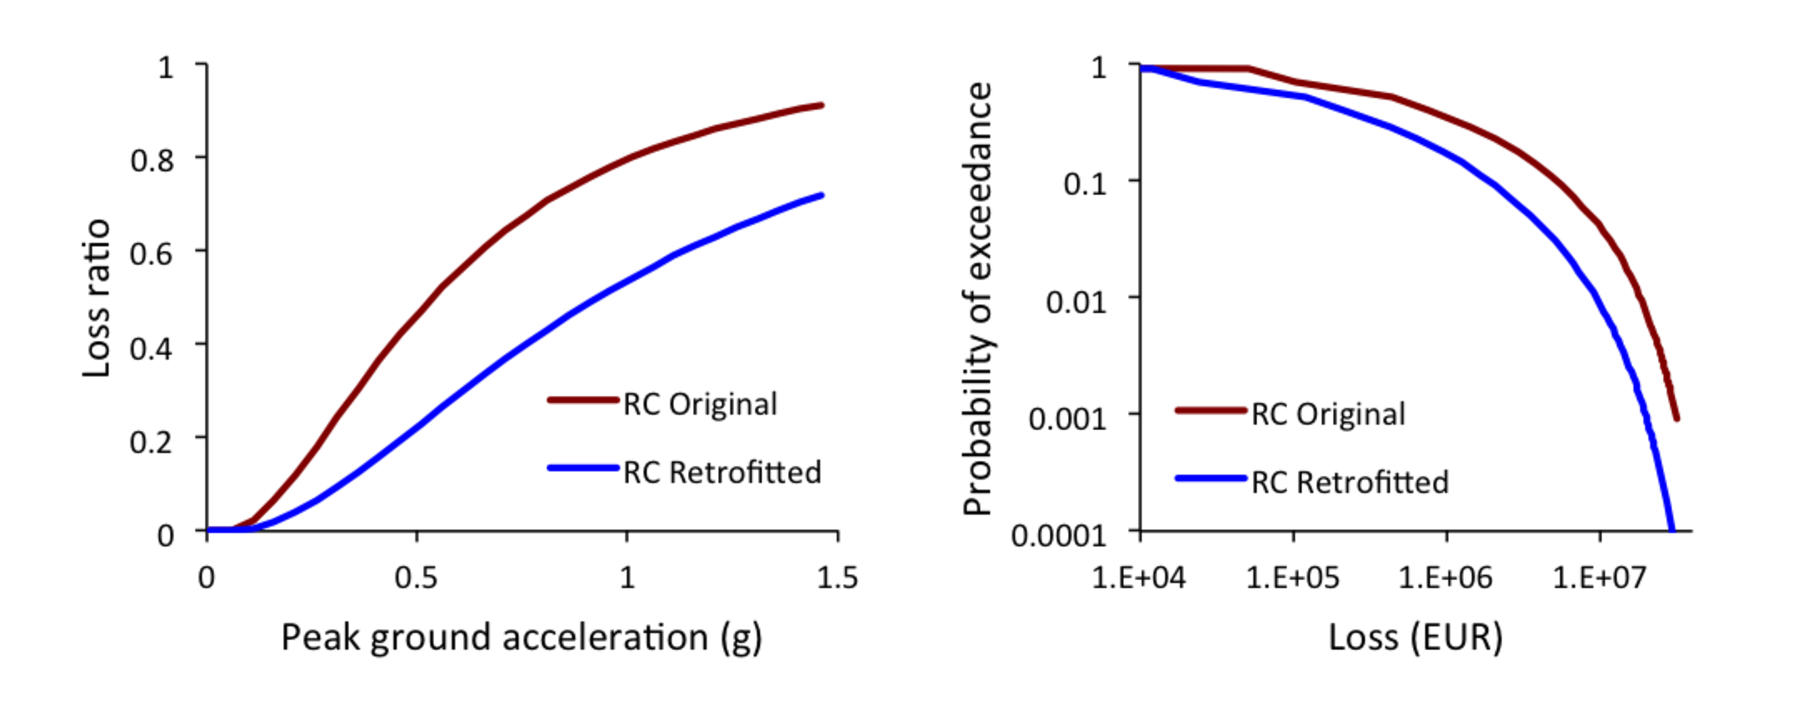
\includegraphics[width=12cm,height=5cm]{./figures/risk/VulnerabilityLosscurve.eps}
\caption{Vulnerability functions for the original and retrofitted configuration of a class of RC buildings (left) and respective loss exceedance curves (right).}
\label{fig:VulLosscurve}
\end{figure}

\item Then, an average annual loss ($AAL$) for each vulnerability configuration is calculated by numerically integrating the respective loss exceedance curve.  

\item For the calculation of the economic benefit $B$, the following formula can be employed:

\begin{equation}
B=(AAL_{retrofitted}-AAL_{original})\times\frac{1-e^{rt}}{r}
\end{equation}

where $r$ represents the inflation rate, which serves the purposes of considering the variation of the economic value of the \glspl{asset} during their life expectancy, or design life ($t$).

\item Finally, the previously defined benefit ($B$) is divided by the retrofitting cost ($C$), leading to the benefit/cost ratio ($BCR$). This process is repeated for all the \glspl{asset} comprised in the \gls{exposure model}.

\end{enumerate}

\section{Calculator Output}
The results of this calculator are stored in a benefit/cost ratio map, which includes the $AAL_{retrofitted}$, $AAL_{original}$ and the resulting $BCR$ at each location. In Figure \ref{fig:BCRMap}, a map of benefit/cost ratios for RC residential buildings in Nepal is presented.

\begin{figure}[ht]
\centering
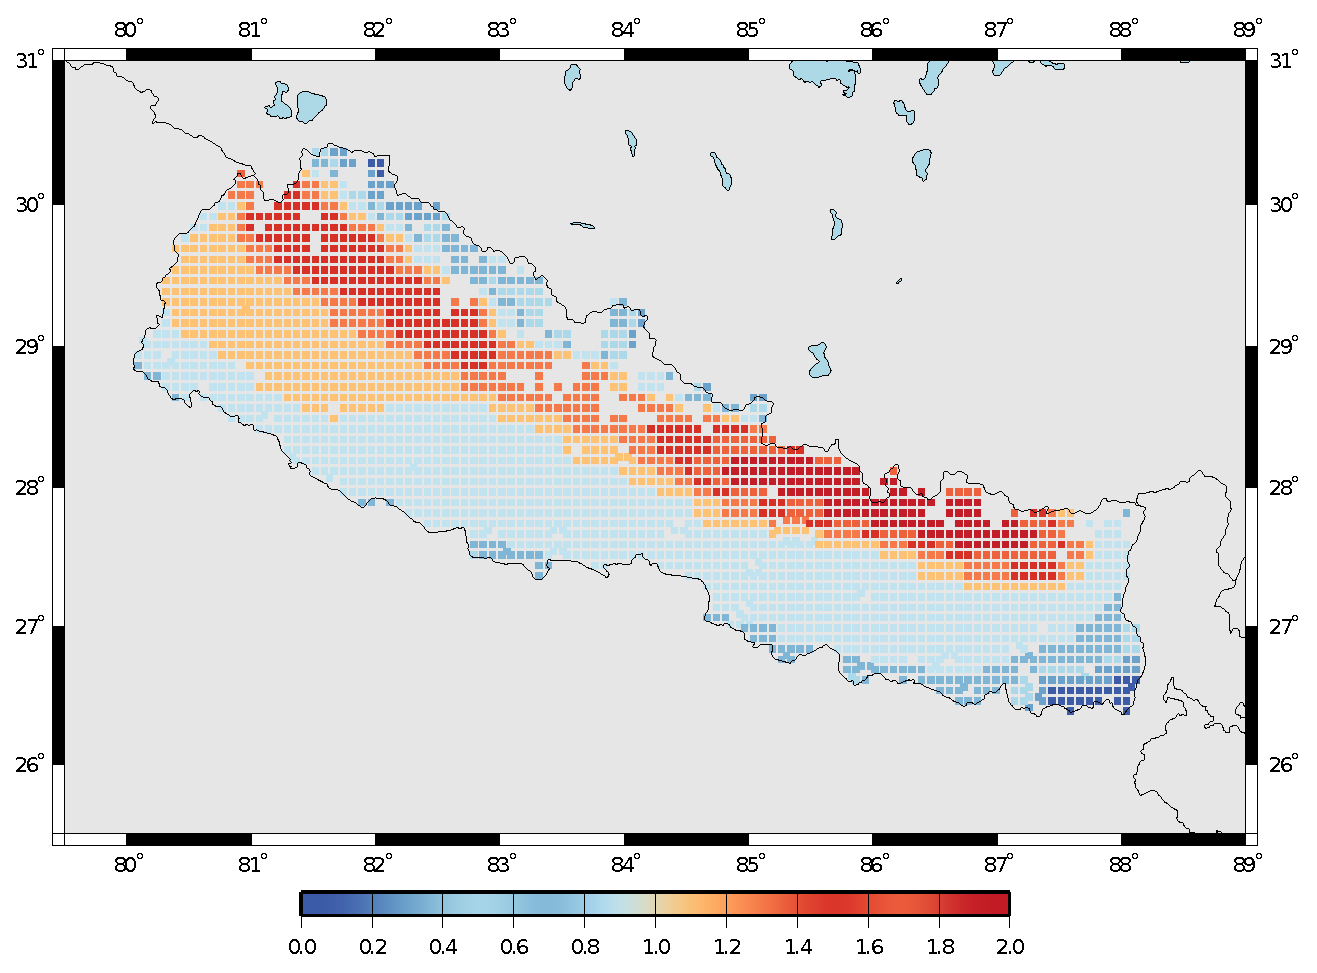
\includegraphics[width=12cm,height=8cm]{./figures/risk/BenefitCostRatioMap.eps}
\caption{Retrofitting benefit/cost ratio map for residential buildings in Nepal.}
\label{fig:BCRMap}
\end{figure}